\section{Motivation}
The non-existent price recovery of the Western Canadian Select crude index since its collapse in 2015 has forced many Canadian energy companies to shift their operating strategies from expansion to optimization \cite{oil_price}.  Typically, existing processes in the oil and gas sector are old and have been operating in a similar regime for many years.  In doing so, vast amounts of data have been collected for the current operating regime.  Through rapid advancements of computer hardware, this data can now be leveraged as a gold mine for modern data hungry machine learning algorithms.  Firstly, the data can be used for predictive applications such as forecasting, digital twinning, soft sensing, and even training purposes.  The data can also be leveraged to create "ML-assisted" safety applications similar to driver assistance in the automotive industry. For example, process monitoring and process forecasting ML models can be built to \textit{proactively} manage operational risk by identifying hazards well in advance of actual incidents. Modern optimal control methods (i.e., maximizing profits of a plant or minimizing operating cost) can also benefit greatly through the assistance of ML algorithms.  Currently, a common optimal control method is MPC; however, the method assumes the availability of an accurate process model.  In any industrial scale process, an accurate process model is nearly impossible to identify due to the vast amount of non-linear interaction effects.  Even after identification, the model would need re-tuning after several months due to process drifts and other changes. Furthermore, for large processes, the dimension of the states and actions may be too large for online optimization to be feasible. One field of study called distributed MPC aims to solve this computational hurdle by decomposing the system into smaller sub-systems; however, distributed MPC performance are typically subpar compared to its centralized counterpart due to communication issues \cite{distributed_mpc}. Through RL, such large problems may be computationally feasible as a centralized algorithm by pre-computing the optimal control policies offline. Moreover, process drifts can be naturally handled by RL through its direct adaptive optimal control nature \cite{direct_adaptive}.  For traditional optimal control, adaptive characteristics are typically indirect and require re-identification of the system models.  In the case of RL, the policy is  adapted directly through interactions with the environment. Although there exists numerous machine learning success stories in the technology sector, their applications in the process industry is still severely limited. One main reason for the absence of recent ML progress is the lack of a workforce skilled in both ML and process control.

Many technology companies and ML engineers specialized in the technology sector have attempted to fill the gap; however, process control data is exceedingly different compared to traditional image or transactional data.  The data in process control is typically unintuitive, time-series, and are often times unreliable or noisy.  There also exists many time delays in chemical processes and feature engineering is difficult without proper fundamentals of process engineering. Comparatively, the data in the technology sector is often very intuitive and easy to understand.  For example, building a classification algorithm for facial recognition is easier to understand compared to predicting when a pump will fail.  The former only requires an image of the individual or some 3D spatial data corresponding to the individual's facial features. In the latter, there may be thousands of interactions affecting the ultimate outcome of the pump, most of which are impossible to identify through intuition alone. Due to these differences, engineers not specialized in the process sector faced great challenges when attempting to create value in the process industry.

More recently, there has been a surge of ML innovations made by research scientists and AI start-up companies catered towards the process industry.  However, most were never commercialized because the mentality between industry and the engineers were vastly different.  In industry, the ultimate objective is to create shareholder value through risk-managed products; it may be traditional methods or it can be ML.  For the research scientists, the focus is more on the elegance and novelty of the algorithm, no matter the complexity. For industry, such algorithms are difficult to explain to a non-technical audience, have a high cost of ownership for the customer, and are difficult to understand without a team of subject matter experts (which themselves cost a significant amount of money).

Throughout this thesis, the main theme is to introduce easy, cost effective solutions that explicitly considers the following four customer focused values required for successful commercial products \cite{marketing}:
\begin{itemize}
    \item \textbf{Functional value:} Describes the overall usefulness of the product compared to other available products.  For example, a ML anomaly detection algorithm may be far superior compared to other methods if enough data is present.
    \item \textbf{Monetary value:} The cost savings generated from this product (e.g., amount of money saved through using an optimization algorithm or preventing a loss incident).  
    \item \textbf{Social value:} Ability for the product to enhance your brand or product awareness and is especially important for sales focused enterprises.  For example, after an individual goes to Disneyland, they may tell many people how great it was without any incentive from Disney.  In the process industry, operators and/or engineers will recommend great products that helped them in their jobs and/or become more productive without external incentives.
    \item \textbf{Psychological value:} Ability to make the company feel superior compared to the competition.  For example, a firm may believe they have better chances at winning contracts if their products contain state-of-the-art ML technology needed for big data applications.
\end{itemize}
Ultimately, the goal is to create organic growth for the local industry through new, innovative ways.  If an exceptionally complex solution is engineered, but there exists no customers, the solution didn't end up solving anything. This thesis introduces novel techniques to cater machine learning to the local industry, ranging from commodities transportation to automation.

\section{Introduction to AI}
Artificial intelligence (AI) has set off a change in perspective in the various sectors around the globe, ranging from health care to manufacturing.  The previously arcane topic is now spreading wildly across countless academic and industrial minds alike. Quick progressions in computing power and declining prices in data storage combined with AI's self-learning abilities has transcended the elevated AI to become the go-to algorithm for many difficult worldwide problems such as natural language processing, predictive analytics, and computer vision.  PwC projected AI to contribute well over \$15 trillion USD to the global economy by 2030, while elevating GDP of local markets by 26\%  \cite{pwc}. Generally speaking, the field of AI is ever-expanding and contains many goals.

Figure \ref{fig:AIGoals} shows the six major goals of AI.  Out of all the goals, machine learning (ML) is currently the most influential topic in industry.  The field of ML can be described as the study that develops algorithms to give machines explicit abilities to learn different tasks without being pre-programmed to do so \cite{AI}.  ML can be further decomposed into supervised learning, unsupervised learning, semi-supervised learning (a combination of supervised and unsupervised learning), and reinforcement learning.

\begin{figure}[H]
    \centering
    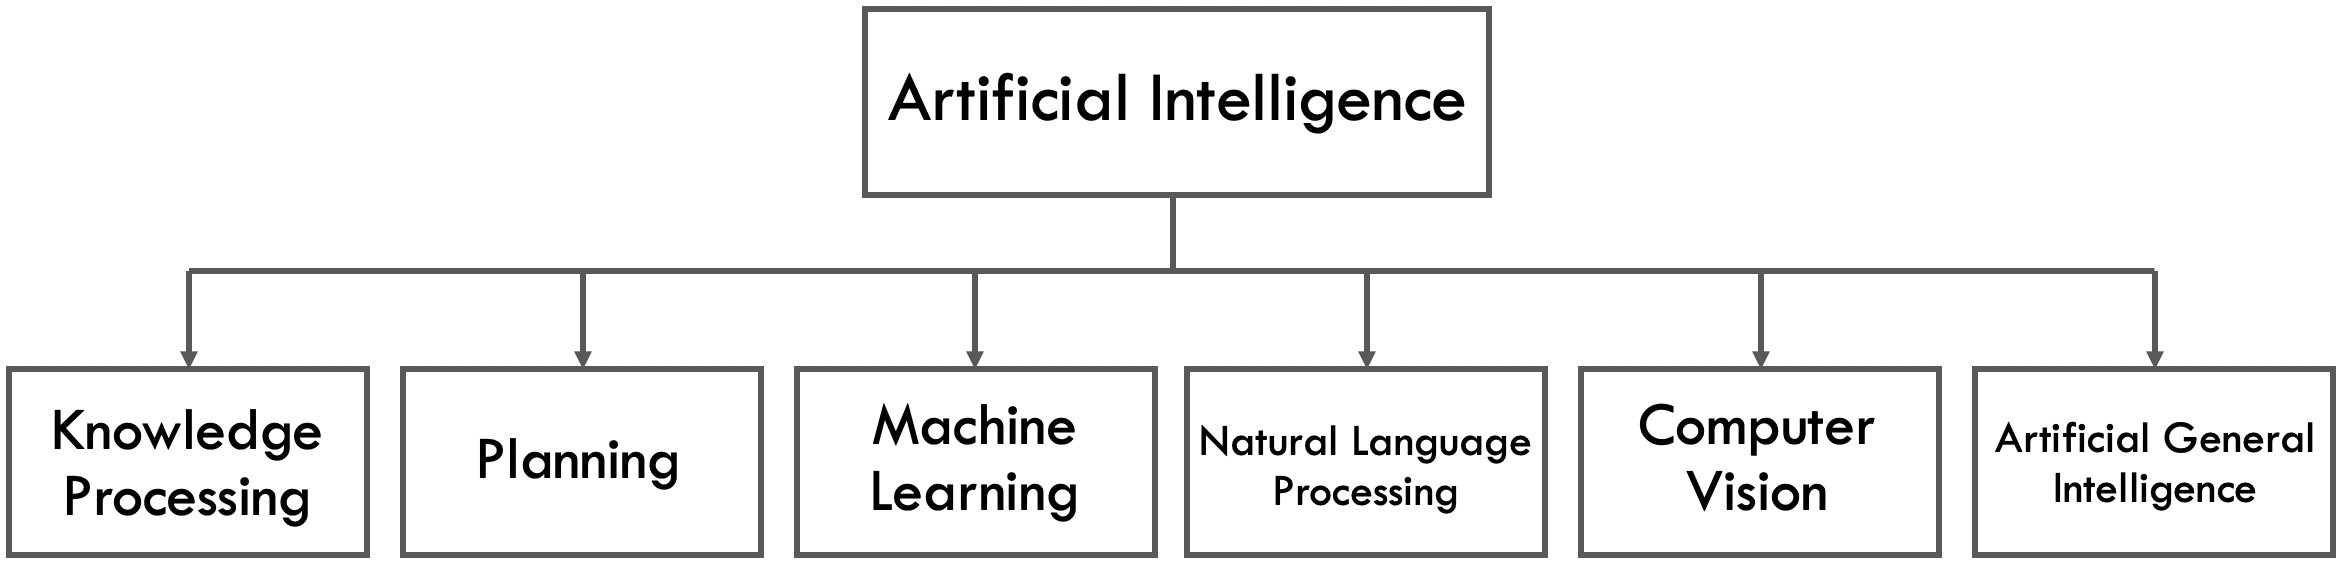
\includegraphics[width=\textwidth]{images/ch1/AIGoals.jpeg}
    \caption{The major goals of artificial intelligence.}
    \label{fig:AIGoals}
\end{figure}   

The sub-fields of ML are shown in Figure \ref{fig:MLGoals}.  In supervised learning, the algorithm learns the optimal input-output mapping, called the model, from a training data set pre-labeled by an external supervisor \cite{sutton}.  Be aware that not all labels provided are guaranteed to be correct. In fact, it is not uncommon to  have mislabeled data caused by noise in the original data set. For example, imagine trying to transcribe an interview with the audio playback heavily corrupted by noise.  In the process industry, the supervisor is typically a sensor measuring the current condition of the process (pressure, temperature, flow rate, etc.) and are often times unreliable. In the end, the performance of the supervised learning model is \textit{upper bounded} by the quality of the labels provided by the supervisor.  In the ideal case, the model can exactly replicate the right \textit{and wrong} labels of the supervisor. In unsupervised learning, the algorithms are typically used to optimally segregate data based on their similarity or to identify the principal components within large data sets \cite{Hinton, sutton}.  Objectively, unsupervised learning identifies hidden patterns within data sets through feature extraction and dimensional reduction. Semi-supervised learning is a hybrid between supervised and unsupervised learning where the models are trained on a small data set of labeled data and refined using features extracted from the unlabeled data set. For example, in the process industry, tasking an engineer to manually label data sets is a costly but required endeavor.  In many applications such as fault detection or root cause analysis, a well labeled data set is required to materialize any useful applications.  Using semi-supervised learning in these scenarios, the model can learn from the small labeled data set and extract additional helpful insights from the remaining unlabeled data to fine tune performance.  In this case, the final algorithm is vastly superior compared to its supervised or unsupervised learning counterpart \cite{machine_learning}.  Unfortunately, all the above methods exhibit one critical flaw: \textit{the inability to transcend the supervisor in terms of performance}. Although these methods may provide great cost reductions and/or greatly speed up production through automating trivial tasks, the methods fail to expand the current capabilities of modern methods.

\begin{figure}[H]
    \centering
    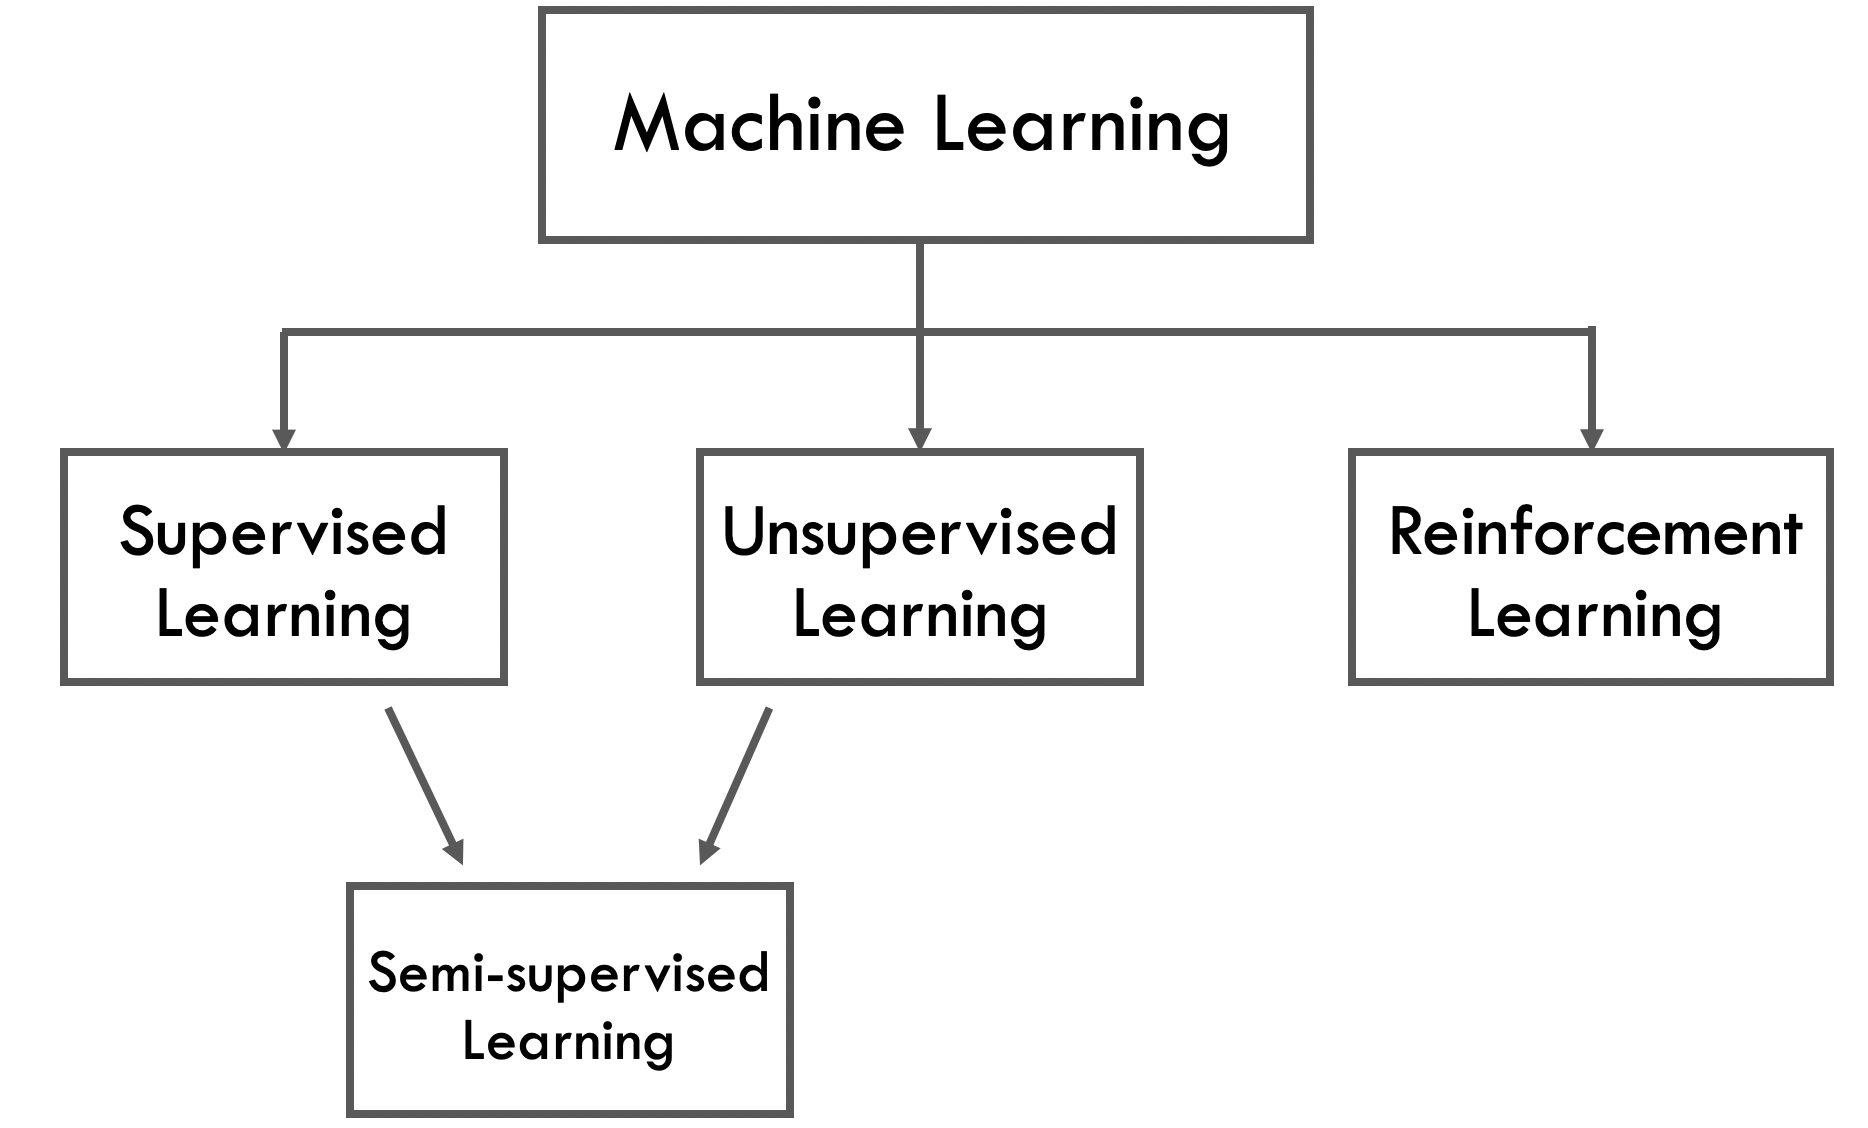
\includegraphics[width=0.6\textwidth]{images/ch1/MLGoals.jpeg}
    \caption{The sub-components of machine learning.}
    \label{fig:MLGoals}
\end{figure}   

Reinforcement learning (RL) aims to overcome this dilemma by providing machines the ability to \textit{surpass all known methods}.  More specifically, reinforcement learning \textit{agents} learns the optimal actions to perform in different situations (also called optimal policy) through self-interaction with the environment.  After each interaction, the agent is provided feedback via a scalar reward signal; large positive rewards follow good actions while negative rewards follow bad actions.  In challenging circumstances, actions affect both the immediate reward signal and the subsequent rewards there-forth. In an intuitively context, pursing an University degree may yield negative immediate rewards; however, rewards years down the line may become significantly more positive due to the newly equipped knowledge.  These two characteristics---delayed feedback and guided trial-and-error search---differentiate RL from all other types of algorithms and ultimately permit RL to push the existing boundaries of known science \cite{sutton}.

\section{Thesis Outline and Contributions}
The thesis is organized as follows: First, basic concepts of RL and MPC will be introduced.  In Chapter 2, applications of ML algorithms in prediction applications will be explored on an industrial pipeline.  Following that, ML for process safety applications will be shown in Chapter 3. Safety applications include topics such as anomaly detection, anomaly prediction, and alarm management. Up until Chapter 3, the projects will use exclusively traditional supervised, unsupervised, and semi-supervised learning methods because the applications are predictive in nature.  Towards the end of Chapter 3 until the end of the thesis, RL methods will be introduced because these applications are more control oriented. Chapter 4 contain various different RL applications in process control. Applications here include the optimal control of a waste water treatment plant, set point tracking control of small scale systems, and fault-tolerant control of an industrial distillation tower. Additionally, RL is also compared to MPC on simple small-scale systems in this chapter. Finally, this thesis is concluded in Chapter 5.  A comprehensive project report for the pipeline optimization project introduced throughout this thesis is shown in Appendix A.

The contributions of this thesis is as follows: In Chapter 2, methods for identifying representative process models in an industrial settings are introduced. Additionally, a new adaptive modelling method was formulated here to significantly reduce the cost of ownership of the machine learning models for the industrial partner. The adaptive method also overcomes catastrophic interference and can be retrofitted onto all model structures. Chapter 3 introduces novel data pre-processing approaches to anomaly detection and prediction in the process industry.  Additionally, a new RL-powered alarm management method is introduced for filtering of nuisance alarms, alarm reduction, and alarm prioritization.  Chapter 4 provide comparisons between traditional optimal control methods with RL on many different systems. Furthermore, a new easy-to-implement continuous non-linear RL method is also shown here.  The last contribution in Chapter 4 is the extension of RL into a fault-tolerant control where RL is used for both the fault detection algorithm and the fault tolerant controller. 


%%%%%%%%%%%%%%%%%%%%%%%%%%%%%%%%%%%%%%%%%%%%%%%%%%%%%%%%%%%%%%%%%%%%%%%%%%%%%%%%%%%%%
% Bandits
%%%%%%%%%%%%%%%%%%%%%%%%%%%%%%%%%%%%%%%%%%%%%%%%%%%%%%%%%%%%%%%%%%%%%%%%%%%%%%%%%%%%%

%%%%%%%%%%%%%%%%%%%%%%%%%%%%%%%%%%%%%%%%%%%%%%%%%%%%%%%%%%%%%%%%%%%%%%%%%%%%%%%%%%%%%
% Bandits
%%%%%%%%%%%%%%%%%%%%%%%%%%%%%%%%%%%%%%%%%%%%%%%%%%%%%%%%%%%%%%%%%%%%%%%%%%%%%%%%%%%%%

\section{Preliminaries to Reinforcement Learning}

Reinforcement learning is a goal-directed learning algorithm which continually improves its own performance through interactions with the environment \cite{sutton}. The main objectives of reinforcement learning are to identify hidden structures within the environment and to find the optimal policy (i.e., optimal state to control action mapping) through guidance from an internal scalar reward (feedback). Two distinct characteristics that deviate reinforcement learning from other methods are its trial \& error search to find the optimal policy, and its ability to identify delayed reward signals. Modern reinforcement learning methods combine principles of optimal control and learning methods together to solve for the optimal control trajectory in an environment.  In the remaining sections of this chapter, fundamental reinforcement learning concepts will be introduced.  Then, tabular based RL methods will be shown.  However, due to the "curse of dimensionality" of high dimensional problems, tabular based approaches struggle in large multi-variate scenarios.  To overcome these issues, deep neural networks will be leveraged for function approximation, and deep reinforcement learning will be introduced.

\subsection{A historical overview}
Reinforcement learning is a combination of two fields of research: \textbf{optimal control} through extremizing an objective function through dynamic programming and \textbf{animal psychology} inspiring trial-and-error search. Originally, the \textbf{optimal control} problem was proposed for designing controller to maximize or minimize the objective function of a dynamical system over time \cite{mpc}.  By the 1950s, Richard Bellman extended on the works of Hamilton and Jacobi to develop a novel approach to solve the optimal control problem.  This approach, known as dynamic programming, optimizes a system's input trajectory by using the functional equation (a function where the unknowns are also functions) generated from the system's state information together with a value function \cite{bellman1}.  The functional equation, now called the Bellman equation, is mathematically represented as:
% Will leave spaces during submission for reviewers
\begin{equation}
    V(x) = r(x) + \gamma \sum P(x' | x, u) \cdot V(x')
    \label{eq:bellman_eq}
\end{equation}
where $V(x)$ represents the value function of $x$. Here, $\gamma$ denotes the discount factor to incorporate future uncertainty. $r(x)$ is the reward signal obtained as a function of the system's desired performance. $P(x'|x, u)$ is the dynamics function describing the transitional probability of arriving at state, $x'$, given $x$ and $u$. $V(x')$ is the value function of $x'$. Intuitively, the value function describes how good or how bad being in particular state is, assuming optimal behaviour thereafter; high values represent good states and low values for bad.  True dynamic programming is "cursed by dimensionality" (i.e., computational cost increases exponentially with the dimensions of the states and actions); thus, approximate dynamic programming (ADP) methods were developed to bypass this hurdle \cite{adp}.  In reinforcement learning, many ADP methods are leveraged to solve for the optimal policy. The concept of a feedback oriented learning system in RL originated from \textbf{animal psychology}. More specifically, the original concept was introduced in the early $20^{th}$ century, named the "Law of Effect". The law stated that animals tend to repeat actions resulting in good outcomes, vice versa for actions with bad outcomes \cite{thorndike}. Initially, the agent explores the environment in which it exists to identify the outcomes corresponding to different actions, then only repeating the actions resulting in good outcomes thereafter. By unifying dynamic programming from optimal control and trial-and-error search from animal psychology, the modern field of RL was developed. For a more comprehensive overview of the history of RL, see \cite{sutton}.

The development of RL is shown in Table \ref{tab:RLevo}.  Reinforcement learning takes its roots from the \textit{k}-armed bandit problem that has been extensively studied in engineering, psychology, and statistics.  This problem disregards state information, and only worries about solving the optimal actions for \textit{one} specific situation \cite{thompson1, thompson2, robbins, bellman_bandit}.  As a natural extension, Barto, Sutton and Brouwer expanded the idea to multi-situation systems \cite{bartosuttonbrouwer} through associative search, also known as \textit{contextual bandits}. The main objective of this algorithm was to find an optimal policy, $\pi^*(x)$, for each situation.  However, it only concerns the immediate rewards and not the long term consequences. Reinforcement learning was then developed to find the optimal policy for different situations based on immediate reward and the onward trajectory there-forth.  

\begin{table}[H]
\caption{From left to right, the evolution of reinforcement learning.}
\centering
\begin{tabular}{c|c|c}
\textbf{$k$-armed bandits}	& \textbf{Contextual bandits}	& \textbf{Reinforcement learning}\\
\hline
Optimal action		  & Optimal action			& Optimal action \\
One situation		  & Many situations			& Many situations \\
Immediate consequence & Immediate consequence	& Long-term consequence \\
\end{tabular}
\label{tab:RLevo}
\end{table}

\subsubsection{\textit{k}-armed Bandit}

The \textit{k}-armed bandit problem provides the fundamentals to understanding modern reinforcement learning.  Here, an agent is present and must choose action $u$ from $\mathcal{U}$, where $\mathcal{U}$ has $k$ choices.  After each action, a scalar reward from a stationary distribution will be returned to the agent as feedback. Favorable actions yield positive rewards, while unfavorable actions return negative rewards. The objective of the agent is to ultimately maximize reward over $N$ steps.  For each action, there is an expected reward called \textit{value}, given by Equation \ref{eq:01value}.

\begin{equation}
    \centering
    q_*(u) = \mathbb{E}[R_t | U_t = u]
    \label{eq:01value}
\end{equation}
where $u$ is the action taken at time, $t$.  $R_t$ is a scalar reward returned to the agent after action $u$ was performed at time $t$. $R_t$ is drawn from a stationary distribution, $R_t \thicksim N(q_*(u), \sigma^2)$. Finally, $q_*(u)$ is the expected reward of taking action, $u$.

The real value is unknown, however, an estimation can be computed and is denoted as $Q_t(u)$.  Given all $Q_t(u)$ is maintained, at any time, one $Q_t(u)$ will be greater than all others. Picking the action that corresponds to the maximum $Q_t(u)$ is known as \textit{greedy}, and the agent is said to be \textit{exploiting}.  If a non-maximum action is picked, the agent is \textit{exploring} \cite{sutton}.

Action selection based on estimating the value of actions are called \textbf{Action-value methods} \cite{action_value_method}. At time $t$, the estimate of the value is given by Equation \ref{eq: value_est} \cite{sutton}.

\begin{equation}
    \centering
    Q_t(u) = \
    = \frac{\sum_{i=1}^{t - 1} R_i \mathbbm{1}_{U_i=u}}
    {\sum_{i = 1}^{t - 1} \mathbbm{1}_{U_i = u}}
    \label{eq: value_est}
\end{equation}
where $\mathbbm{1}$ equals 1 if the condition is true, else 0.  $R_i$ is the reward obtained at the $i^{th}$ episode through selecting action, $U_i$.  Intuitively, the numerator is the sum of rewards when action, $u$, was taken prior to $t$.  Likewise, the denominator is the number of times action, $u$, was taken prior to $t$. As $t \rightarrow \infty$, $Q_t(u) \rightarrow q_*(u)$.  Action selection is based on Equation \ref{eq: bandit_action_selection}.

\begin{equation}
    \centering
    U_t = \argmax_u Q_t(u)
    \label{eq: bandit_action_selection}
\end{equation}

However, initial successful episodes may cause the agent to be stuck at local minimums. To overcome this, a semi-stochastic action selection method called $\epsilon$-greedy can be introduced to promote exploration. In this method, the agent will perform a random action with $\epsilon$ probability (greedy action can be performed).  Higher $\epsilon$ results in more exploratory moves.  Consequently, all $u \in \mathcal{U}$ will be picked many times and by the law of large numbers, $Q_t(a) \rightarrow q_*(a)$ \cite{large_numbers}. Figure \ref{fig: eps_figure} shows the effect of $\epsilon$ on the performance of the agent.

\begin{figure}[H]
    \centering
    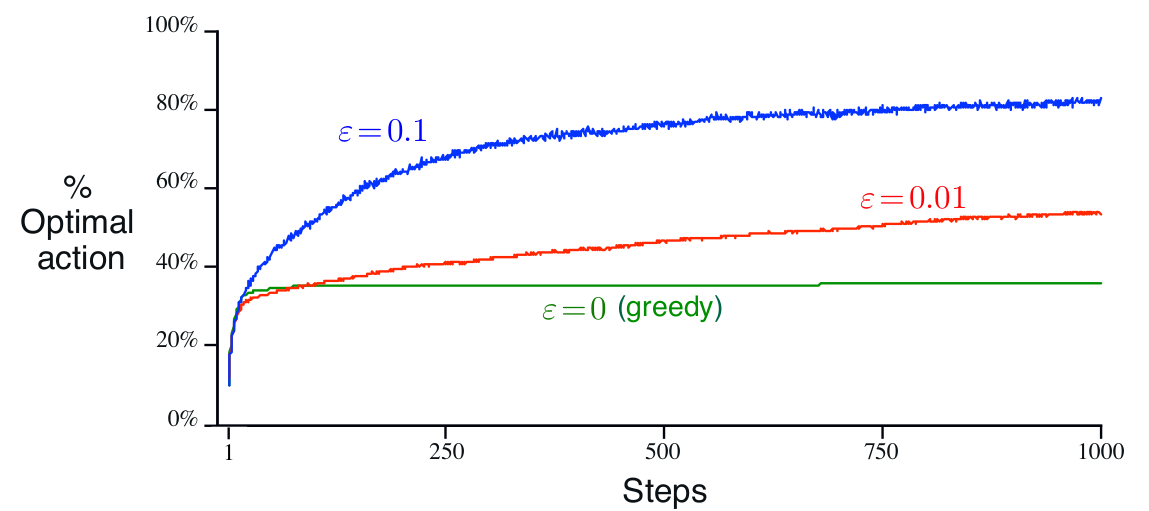
\includegraphics[scale=0.35]{images/eps_vs_optAction.png}
    \caption{Average performance of three agents using different $\epsilon$.  The data is averaged over 2000 runs.  Figure from \textit{Reinforcement Learning: An Introduction} by Sutton and Barto (2018).}
    \label{fig: eps_figure}
\end{figure}

During implementation, $\epsilon$ should decay out as $Q_t(a)$ approaches $q_*(a)$ to ensure knowledge of the agent is being adequately exploited. For non-stationary problems, $\epsilon > 0 \; \forall t$ to ensure other action values have not changed.

Algorithms to solve the \textit{k}-armed bandit problem are easily applied to situations where the concept of state is inert and only the actions are of concern;  a near impossibility in the real world.  

\subsubsection{Contextual Bandit}

A natural extension of the \textit{k}-armed bandit is associative search.  In associative search (sometimes called contextual bandit), different policies are associated with different situations \cite{bartosuttonbrouwer}.  Equation \ref{eq: state-action-value} is the extension of Equation \ref{eq:01value} in the associative search problem.

\begin{equation}
    \centering
    q_*(x, u) = \mathbb{E}[R_t | X_t = x, U_t = u]
    \label{eq: state-action-value}
\end{equation}

Associative search is known as the method between \textit{k}-armed bandits and reinforcement learning.  In associative search, the objective is to associate optimal policies to different situations, but only maximizing the \textit{immediate} reward.  Often times, near term sacrifices are required to initiate the trajectory to a large lump sum reward at the terminal state.  For example, heavy capital and time investment is required for University in the short term.  However, the long term gain is so great that it outweighs the short term losses, making going to University an optimal policy for many individuals.

In order to find the true optimal policy (i.e., policy that returns the greatest rewards over a long time period), the topic of reinforcement learning is developed.  In reinforcement learning, sequential decision making is explored to identify the delayed reward signals from different actions and to ultimately find the optimal policy, $\pi^*$.  

%%%%%%%%%%%%%%%%%%%%%%%%%%%%%%%%%%%%%%%%%%%%%%%%%%%%%%%%%%%%%%%%%%%%%%%%%%%%%%%%%%%%%
% MARKOV DECISION PROCESSES
%%%%%%%%%%%%%%%%%%%%%%%%%%%%%%%%%%%%%%%%%%%%%%%%%%%%%%%%%%%%%%%%%%%%%%%%%%%%%%%%%%%%%

%%%%%%%%%%%%%%%%%%%%%%%%%%%%%%%%%%%%%%%%%%%%%%%%%%%%%%%%%%%%%%%%%%%%%%%%%%%%%%%%%%%%%
% MARKOV DECISION PROCESSES
%
% Introduction to MDPs, finite MDPs, infinite MDPs
% Semi MDPs
% Partially Observable MDPs
%
%%%%%%%%%%%%%%%%%%%%%%%%%%%%%%%%%%%%%%%%%%%%%%%%%%%%%%%%%%%%%%%%%%%%%%%%%%%%%%%%%%%%%

\section{Markov Decision Processes}
In the face of uncertainty, the agent's \textit{sequential} decision making is formalized in the Markov decision process (MDP). The general MDP framework is shown in Figure \ref{fig:01mdp} and contains two components: the \textbf{agent} and the \textbf{system}. The \textbf{agent} is a continuously learning decision maker and is mathematically represented by the RL algorithm. Objectively, the agent will undergo numerous meaningful interactions with the system to ultimately learn the optimal policy, $\pi^*$ (i.e., the optimal decisions given different situations). Conversely, the \textbf{system} contains all elements the agent cannot arbitrarily control. In process control, the ambient temperature, actuators, and even the wires transporting the control signals are all part of the system because the agent cannot \textit{deterministically} manipulate them. 

\begin{figure}[H]
    \centering
    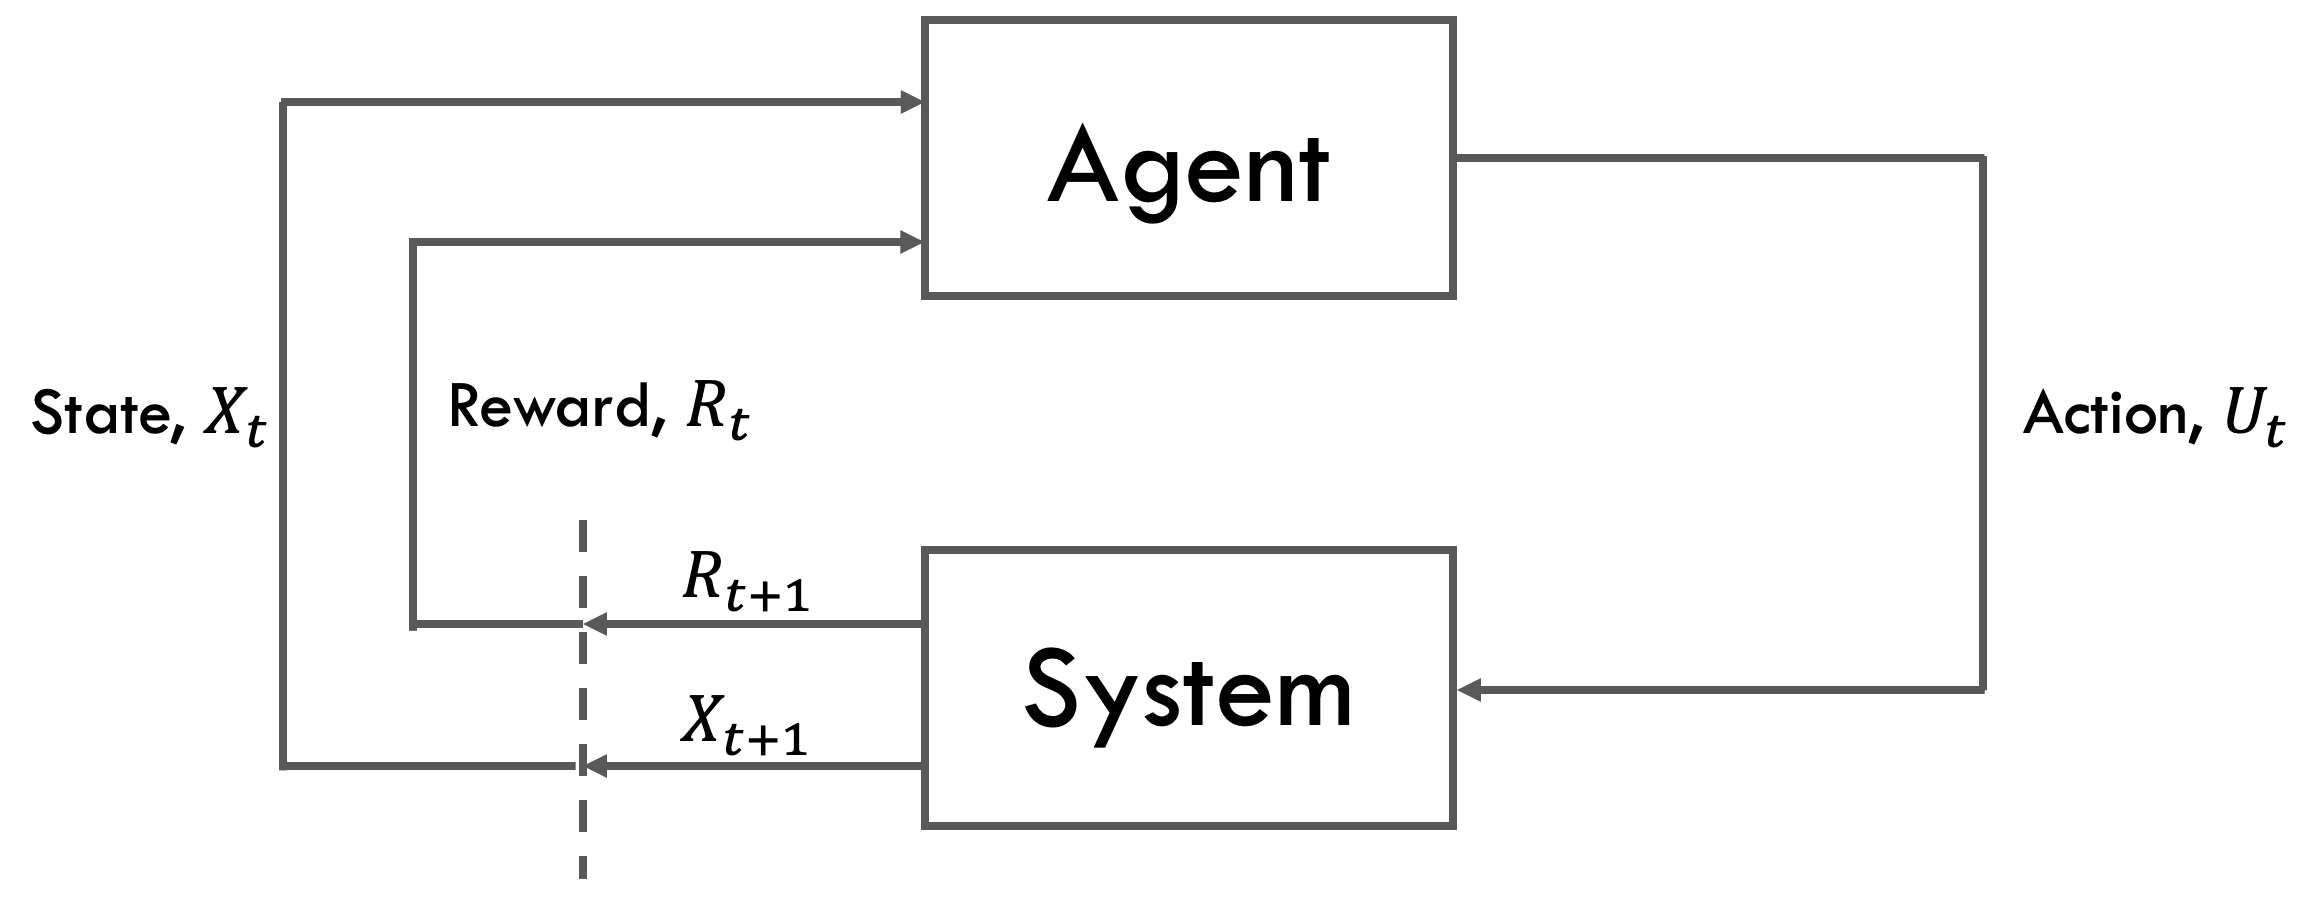
\includegraphics[width=0.56\textwidth]{images/ch1/MDP.jpeg}
    \caption{The general Markov decision process framework. Original image from \cite{sutton}.}
    \label{fig:01mdp}
\end{figure}   

Mathematically, the MDP is a discrete representation of the stochastic optimal problem and a classical formulation of \textit{sequential} decision making where both the immediate and long term consequences are explicitly considered \cite{bellman1, mdp_bellman}. Many definitions of the MDP exist and are equivalent up to small alterations of the process.  One comprehensive definition is that a MDP is a tuple $\mathcal{M}$, is a tuple $(\mathcal{X}, \mathcal{U}$, $P(x', r|x, u), \gamma, R)$ comprised of the following\cite{ng_ref12}:
\begin{itemize}
    \item $x \in \mathcal{X}$: \textbf{State} space of the system at each time step. Common states in industrial processes include temperatures, valve positions, pressures, flow rates, etc.
    \item $u \in \mathcal{U}$: Bounded \textbf{action} space of the agent, ($\mathcal{U}$ $ \geq 2 $). In traditional control, this is the \textbf{bounded input signals} sent to the actuators.
    \item $R \in \mathbb{R}$: Expected \textbf{reward} signal after performing action $u$ in state $x$. Reward functions are designed based on a desired performance metric.  In control theory, the reward function is known as the \textbf{objective function}.  Typically, $|R| \leq \mathcal{R}$ for convergence guarantees.
    \item $p(x', r|x, u)$: Systems \textbf{dynamics function}. Formally, it is the probability of transitioning to $x'$ and receiving $r$,  given states $x \in \mathcal{X}$ and performing action $u \in \mathcal{U}$. Mathematically, it is described by the following:
    \begin{equation}
        p(x', r | x, u) \dot{=} Pr\{X_t = x', R_t = r | X_{t - 1} = x, U_{t-1} = u\}
        \label{eq:transition_prob}
    \end{equation}
    where $p$ describes the system \textbf{dynamics} and $Pr$ denotes the probability operation \cite{sutton}. Additionally, $p$ satisfies the following equality:
    \begin{equation}
        \sum\limits_{x' \in \mathcal{X}} \sum\limits_{r \in \mathcal{R}} p(x', r | x, u) = 1, \forall x \in \mathcal{X}, u \in \mathcal{U}
        \label{eq:prob}
    \end{equation}
    Notice here that $p$ is only a function of the \textit{immediate past}, thus assuming that $x_{t - 1}$ and $u_{t-1}$ captures the complete history. This is known as the Markov property and its underlining assumptions are critical for successful process control applications using RL. Additionally, note that when the state and actions are formulated as augmented past information: $x_{t-1} = [s_{t-1}, s_{t-2}, ... s_{t-N}], u_{t-1} = [a_{t-1}, a_{t-2}, ..., a_{t-N}]$, where $s_{t-N}$ and $a_{t-N}$ denotes the past states and actions, the system is still Markov because decisions can be made exclusively using $x_{t-1}$ and $u_{t-1}$. 
    \item $\gamma$: \textbf{Discount factor} associated with uncertainty of the future, ($0 \leq \gamma \leq 1)$. $\gamma < 1$ is also a requirement for continuous processes to guarantee eventual convergence.
\end{itemize}

There exists three different MDPs: fully observable MDP (FOMDP), partially observable MDP (POMDP), and semi MDP (SMDP). Table \ref{tab:01mdps} shows a general guideline on the different MDPs.

\begin{table}[H]
\caption{A comparison of different Markov decision processes.}
\centering
\begin{tabular}{c|c|c}
\textbf{FO-MDPs}	& \textbf{S-MDPs}	& \textbf{PO-MDPs}\\
\hline
All states observable		  & All states observable			& Some states observable \\
Discrete time		          & Continuous time	             	& Discrete time \\
\end{tabular}
\label{tab:01mdps}
\end{table}

\subsection{Fully observable Markov decision processes}
Fully observable Markov decision processes are the simplest and serves as the foundational framework.  They are mainly applied to discrete systems with fixed sampling times where transition dynamics are unimportant and all states are observable (measurable in control literature). Here, the agent starts in some initial states, $x_0$. At each time $t$, the agent maps $x_t$ to some $u_t$ corresponding to its policy, $\pi_t$.  Given $x_t$ and $u_t$, the system will then transition to some new states $x_{t+1}$ dictated by Equation \ref{eq:transition_prob} while outputting reward signal $R_{t+1}$ based on the reward function. In regulation and set-point tracking problems, this reward function is typically the squared tracking error between $x_t$ and $x_{sp}$.  By repeating this cycle many times, the agent is able to traverse through some sequence, $x_t, u_t, R_{t+1}, x_{t+1}, u_{t+1}, R_{t+2}, x_{t+3}, ...$ and accumulate \cite{sutton}:
\begin{align}
G_t &= R_{t+1} + \gamma R_{t+2} + \gamma^2 R_{t+3} ... \\
    &= \sum\limits^{\infty}_{k = 0} \gamma^k R_{t+k+1}
\label{eq:return}
\end{align}
where $G_t$ denotes the cumulative discounted return at time $t$ and $\gamma$ is the discount factor to capture the future uncertainty. MDPs can represent both finite or infinite systems; the former describes episodic tasks with explicit terminal states while the latter describes tasks that continue forever.  Intuitively, most two-player board games such as Checkers, Chess, or Go are finite MDPs where the game is terminated after one player is defeated.  Contrarily, an infinite MDP system could be the control system in an industrial process. For infinite MDP systems, $\gamma < 1$ is a necessary condition to keep $G_t$ bounded. Ultimately, the agent is tasked with finding the optimal policy, $\pi^*$, that maximize $G_t$, and subsequently the value function, over $N$ steps. The value function for each state is given as \cite{sutton}:
\begin{align}
    v_\pi (x) &\dot{=} \mathbb{E}_\pi [G_t | X_t = x] \\
              &= \mathbb{E}_\pi \left[\sum\limits^\infty_{k=0} \gamma^k R_{t+k+1} | X_t = x \right] \\
              &= \mathbb{E}_\pi [R_{t+1} + \gamma G_{t+1} | X_t = x]
    \label{eq:value_func}
\end{align}
where $v_\pi (x)$ is the value function of $x$ under policy $\pi$. Theoretically, the existence and uniqueness of $v_{\pi}$ is guaranteed for continuous systems where $\gamma < 1$ or in systems with guaranteed termination.  Compared to Equation \ref{eq:01value}, Equation \ref{eq:value_func} takes the expectation of $G_t$; therefore, explicitly optimizing the long term returns rather than only the immediate rewards. The action-value formulation of Equation \ref{eq:value_func} is:
\begin{align}
    q_\pi (x, u) \; &\dot{=} \; \mathbb{E}_\pi [G_t | X_t = x, U_t = u] \\
                 &= \mathbb{E}_\pi \left[\sum\limits^\infty_{k=0} \gamma^k R_{t+k+1} | X_t = x, U_t = u \right], \forall x, u \in \mathcal{X, U}
    \label{eq:a_value_func}
\end{align}
FOMDPs work well for discrete systems where all states are observable.  However, system states in industrial processes are often unobservable (unmeasurable in control) due to limited hardware or engineering limitations. In such systems, the Markov property no longer holds resulting in sub-optimal decision making of the agent.





\subsection{Partially observable Markov decision processes}
Partially observable Markov decision processes (POMDPs) extend upon the concepts of FOMDPs and represent systems with unobservable states. In RL literature, observability is equivalent to measurability in control; thus, the two terms are used interchangeably here-forth. In FOMDPs, the current state $x_t$ at each time $t$ is fully observable. In the more general setting of POMDPs, the entire state vector describing the agent's current situation is no longer available. Instead, the agent only has access to a set of possible observations $\mathcal{O}$. At each time $t$, the agent sees observation $o_t$ which correspond to probability distributions over states.  Using $o_t$, the agent can infer the states it \textit{might} currently be in \cite{ng_ref12}. Relating to a process control setting, existing sensors typically only measure a subset of the current states; however, by using available measurements, one can infer the remaining unmeasurable states using probabilistic approaches.

Generally, finding $\pi^*$ in a POMDP setting is significantly harder compared to FOMDPs.  Even finding a near-optimal policy is at least NP-hard (non-deterministic polynomial time) \cite{pomdp_time}.  Furthermore, even agents with access to all the system's true value functions are unable to behave optimally in a POMDP setting because the current states are unknown \cite{ng_ref12}. 

Belief states is one method for agents to behave optimally in POMDPs. On a high level, belief states transform the POMDP setting into its FOMDP counterpart through a probabilistic approach. Specifically, belief states, $b$, are probability distributions over states deduced using previous observations and actions. The probability distributions represent what the agent thinks its current state is. Using these probabilities, the agent can compute scalar value functions of each state-action pair and use these to act "optimally".  Note here that the agent's behaviour is optimal given the available information, and not optimal with respect to the system. An quantitative example is provided below:
\begin{quote}
    Suppose an agent exists in a two-input two-output (TITO) POMDP setting with two unobservable states ($x_1$ and $x_2$) and two actions ($u_1$ and $u_2$) and suppose the problem is only concerned with the immediate consequences (for longer horizons, the agent must also consider the long term rewards, making the example less intuitive). In this system, there are four value functions, one for each state-action pair. Suppose $u_1$ earns a reward of 2 in $x_1$ and 0 in $x_2$.  Similarily, $u_2$ earns a reward of 0 in $x_1$ and 1 in $x_2$.  Given $b_t = [0.2, 0.8]$ (probabilities of being in $x_1$ and $x_2$, respectively), then $Q(b_t, u_1) = 0.2 \cdot 2 + 0.8 \cdot 0 = 0.4$ and $Q(b_t, u_2) = 0.2 \cdot 0 + 0.8 \cdot 1 = 0.8$, resulting in $u_2$ being the optimal action.
\end{quote}

In control theory, observers, such as soft sensors, are used to estimate unmeasurable states.  Observers are typically $1^{st}$ principles, data driven, or probabilistic models. The concept of belief states is very similar to observer design in control theory. Traditionally, Kalman filter is a widely used observer design. Conversely, recurrent neural networks (RNNs) are widely used for belief state estimation in RL. The performance of RNN was compared with Kalman filter in \cite{RNNvsKF}, drawing similarities of the two methods' objective, theory, and performance.

System representations using FOMDPs and POMDPs work well in discrete tasks where transition times are constant and transition dynamics are disregarded; however, both topics are paramount for continuous optimal control.  







\subsection{Semi Markov decision processes}
Typical MDPs are discrete representations of the optimal control problem and are sub-optimal in continuous tasks. Semi-Markov decision processes (SMDP) are an extension of MDPs to continuing tasks with unknown transition times and system dynamics. In SMDPs, the transition dynamics of the system are explicitly captured using reward function \cite{continuous_rl_ref14}:
\begin{equation}
R(x_t, x_{t+1}, u_t) = \int\limits^\infty_0 \int\limits^t_0 e^{-\beta s} \rho(x_t, \pi (x_t))dsdF_{x_t, x_{t+1}}(t | \pi (x_t))
\label{eq:reward_rate}    
\end{equation}
where $R(x_t, x_{t+1}, u_t)$ is the expected reward to be received when transitioning from $x_t$ to $x_{t+1}$ after action $u_t$. The rewards, $R$, are calculated at each time step in the transition period to explicitly capture transition information. Then, the average reward of the transition is used to update the agent. Here, $\rho(x_t, \pi(x_t))$ represents the average reward during the transition following policy, $\pi$. $F_{x, x_{t+1}}(t, u)$ denotes the probability distribution of the time required to transition from $x_t$ to $x_{t+1}$.  Finally, $\beta > 0$ denotes the \textit{constant} discount factor in SMDPs, where higher $\beta$ results in short-sighted agents. In SMDPs, the discount factor is corrected for transition time during each update step.  The corrected discount factor is given by:
\begin{equation}
    \gamma(x_t, x_{t+1}, u) = \int\limits^{\infty}_0 e^{-\beta t} dF_{x_t, x_{t+1}}(t | \pi_t)
\end{equation}
where $\gamma (x_t, x_{t+1}, u_t)$ is the expected discount factor that will be applied to the value of state $x_{t+1}$ during the update step shown in Equation \ref{eq:bellman_eq}. The value function for SMDPs is obtained from combining Equations \ref{eq:reward_rate} and \ref{eq:value_func}:
\begin{equation}
v_{\pi}(x_t) = \frac{1 - e^{-\beta \tau}}{\beta} R(x_t, x_{t+1}, \pi(x_t)) + e^{-\beta \tau}v_{\pi}(x_{t+1})
\end{equation}
where $\tau$ is the unknown transition time.  Similarily, the action-value form is given by:
\begin{equation}
    q_{\pi}(x_t, u_t) = \frac{1 - e^{-\beta \tau}}{\beta} R(x_t, x_{t+1}, \pi(x_t)) + e^{-\beta \tau}  q_{\pi}(x_{t+1}, u_{t+1})
\end{equation}
By representing control problems as SMDPs, control strategies resulting in large overshoot, inverse response, or any other undesirable dynamics behaviour can be minimized. Additionally, the system will be able to handle systems with unknown transition times.  An intuitive example illustrating the advantages of SMDPs in process control is as follows:

\begin{quote}
    Suppose a refinery company is operating a continuously stirred tank reactor (CSTR). Objectively, the CSTR must maintain 200$^{\circ}$ C for optimal performance.  The temperature is controlled through a heat exchanger using cold water.  A RL agent was built to optimally control the flow of cold water to maintain the temperature set point. Suppose the CSTR starts at 220$^{\circ}$ C.  Agents using MDP representations may be overly aggressive and send large input signals because the reward is only calculated \textit{right before} the next evaluation step. Therefore, input signals resulting in large overshoot or inverse response may not be reflected in the reward. Contrarily, SMDP representation uses the average reward accumulated along the trajectory to provide feedback to the agent, allowing the transition dynamics to be explicitly captured. This way, input signals resulting in undesirable behaviour can be captured and mitigated. Furthermore, SMDP representations can have flexible evaluation times (traditional representations evaluate after a set time period), enabling re-evaluation during the transitional period and adjusts the discount factor in accordance to the elapsed time from last evaluation.
\end{quote}









\subsection{Optimal solution of the Markov decision processes}
The optimal solution to the RL problem refers to identifying a policy that generates the highest long term returns. Such a policy may not be unique; there may exist many optimal policies, where $v_{\pi^*_1} = v_{\pi^*_2} = ... = v_{\pi^*_N}$.  Formally, the optimal policy must satisfy the \textbf{principle of optimality}: the optimal policy $\pi^*$ is optimal if and only if $v_{\pi^*}(x) \geq v_{\pi \neq \pi^*}(x)$ for all $x \in \mathcal{X}$ \cite{PO}. Mathematically, the optimal value function is:
\begin{equation}
    v^*(x) \dot{=} \argmax_{\pi} v_{\pi}(x), \forall x \in \mathcal{X}
\end{equation}
with its action-value variant being:
\begin{equation}
    q^*(x, u) \dot{=} \argmax_{\pi} q_{\pi}(x, u), \forall x, u \in \mathcal{X, U}
\end{equation}
In a more explicit form, the optimal value function and action-value function written in terms of Equations \ref{eq:value_func} and \ref{eq:a_value_func} are given, respectively, by \cite{sutton}:
\begin{equation}
    v^*(x) = \argmax_{u} \mathbb{E}[R_{t+1} + \gamma v^*(X_{t+1}) | X_t = x, U_t = u]
    \label{eq:01valuefunc}
\end{equation}
\begin{equation}
    q^*(x, u) = \mathbb{E}\left[R_{t+1} + \gamma \argmax_{u_{t+1}} q^*(X_{t+1}, u_{t+1}) | X_t = x, U_t = u \right]
\end{equation}
Here, the $max$ operation denotes that the optimal action will be taken for the remaining of the trajectory. Theoretically, all optimal value functions can be explicitly solved using Equation \ref{eq:01valuefunc}; however, such a task would require unreasonable amounts of computation power for even simple systems. In the following section, three popular methods will be introduced to estimate the value and action-value functions in reinforcement learning.


%%%%%%%%%%%%%%%%%%%%%%%%%%%%%%%%%%%%%%%%%%%%%%%%%%%%%%%%%%%%%%%%%%%%%%%%%%%%%%%%%%%%%
% Reinforcement Learning
%%%%%%%%%%%%%%%%%%%%%%%%%%%%%%%%%%%%%%%%%%%%%%%%%%%%%%%%%%%%%%%%%%%%%%%%%%%%%%%%%%%

%%%%%%%%%%%%%%%%%%%%%%%%%%%%%%%%%%%%%%%%%%%%%%%%%%%%%%%%%%%%%%%%%%%%%%%%%%%%%%%%%%%%%
% Reinforcement Learning
%
% Introduction to MDPs, finite MDPs, infinite MDPs
% Semi MDPs
% Partially Observable MDPs
%
%%%%%%%%%%%%%%%%%%%%%%%%%%%%%%%%%%%%%%%%%%%%%%%%%%%%%%%%%%%%%%%%%%%%%%%%%%%%%%%%%%%

\section{Introduction to Reinforcement Learning}

Reinforcement learning is a goal-directed learning algorithm which continually improves its own performance through interactions with the environment \cite{sutton}. The main objectives of reinforcement learning are to identify hidden structures within the environment and to find the optimal policy (i.e., optimal input trajectory) through guidance from an internal scalar reward (feedback). Two distinct characteristics that deviate reinforcement learning from other methods are its trial \& error search to find the optimal policy, and its ability to identify delayed reward signals. Modern reinforcement learning methods combine principles of optimal control and learning methods together to solve for the optimal control trajectory in an environment.  In this chapter, fundamental reinforcement learning concepts are first introduced.  Then, tabular based methods will be shown.  However, due to the "curse of dimensionality" of high dimensional problems, tabular based approaches fail to bear fruit.  To overcome these issues, deep neural networks will be used for function approximation, and deep reinforcement learning will be introduced.

Reinforcement learning takes its roots from the \textit{k}-armed bandit problem that has been extensively studied in engineering, psychology, and statistics.  This problem disregards state information, and only worries about solving the optimal actions for \textit{one} specific situation \cite{thompson1, thompson2, robbins, bellman_bandit}.  As a natural extension, Barto, Sutton and Brouwer expanded the idea to multi-situation systems \cite{bartosuttonbrouwer} through associative search, also known as \textit{contextual bandits}. The main objective of this algorithm was to find an optimal policy, $\pi^*(x)$, for each situation.  However, it only concerns the immediate rewards and not the long term consequences. Reinforcement learning was then developed to find the optimal policy for different situations based on immediate reward and the onward trajectory there-forth.  

\subsubsection{\textit{k}-armed Bandit}

The \textit{k}-armed bandit problem provides the fundamentals to understanding modern reinforcement learning.  Here, an agent is present and must choose action $u$ from $\mathcal{U}$, where $\mathcal{U}$ has $k$ choices.  After each action, a scalar reward from a stationary distribution will be returned to the agent as feedback. Favorable actions yield positive rewards, while unfavorable actions return negative rewards. The objective of the agent is to ultimately maximize reward over $N$ steps.  For each action, there is an expected reward called \textit{value}, given by Equation \ref{eq: value}.

\begin{equation}
    \centering
    q_*(u) = \mathbb{E}[R_t | U_t = u]
    \label{eq: value}
\end{equation}
where $u$ is the action taken at time, $t$.  $R_t$ is a scalar reward returned to the agent after action $u$ was performed at time $t$. $R_t$ is drawn from a stationary distribution (typically Gaussian), $R_t \thicksim N(q_*(u), \sigma^2)$. Finally, $q_*(u)$ is the expected reward of taking action, $u$.

The real value is unknown, however, an estimation can be computed and is denoted as $Q_t(u)$.  Given all $Q_t(u)$ is maintained, at any time, one $Q_t(u)$ will be greater than all others. Picking the action that corresponds to the maximum $Q_t(u)$ is known as \textit{greedy}, and the agent is said to be \textit{exploiting}.  If a non-maximum action is picked, the agent is \textit{exploring} \cite{sutton}.

Action selection based on estimating the value of actions are called \textbf{Action-value methods} \cite{action_value_method}. At time $t$, the estimate of the value is given by Equation \ref{eq: value_est} \cite{sutton}.

\begin{equation}
    \centering
    Q_t(u) = \
    = \frac{\sum_{i=1}^{t - 1} R_i \mathbbm{1}_{U_i=u}}
    {\sum_{i = 1}^{t - 1} \mathbbm{1}_{U_i = u}}
    \label{eq: value_est}
\end{equation}
where $\mathbbm{1}$ equals 1 if the condition is true, else 0.  $R_i$ is the reward obtained at the $i^{th}$ episode through selecting action, $U_i$.  Intuitively, the numerator is the sum of rewards when action, $u$, was taken prior to $t$.  Likewise, the denominator is the number of times action, $u$, was taken prior to $t$. As $t \rightarrow \infty$, $Q_t(u) \rightarrow q_*(u)$.  Action selection is based on Equation \ref{eq: bandit_action_selection}.

\begin{equation}
    \centering
    A_t = \argmax_a Q_t(u)
    \label{eq: bandit_action_selection}
\end{equation}

However, initial successful episodes may cause the agent to be stuck at local minimums. To overcome this, a semi-stochastic action selection method called $\epsilon$-greedy can be introduced to promote exploration. In this method, the agent will perform a random action with $\epsilon$ probability (greedy action can be performed).  Higher $\epsilon$ results in more exploratory moves.  Consequently, all $u \in \mathcal{U}$ will be picked many times and by the law of large numbers, $Q_t(a) \rightarrow q_*(a)$ \cite{large_numbers}. Figure \ref{fig: eps_figure} shows the effect of $\epsilon$ on the performance of the agent.

\begin{figure}[h]
    \centering
    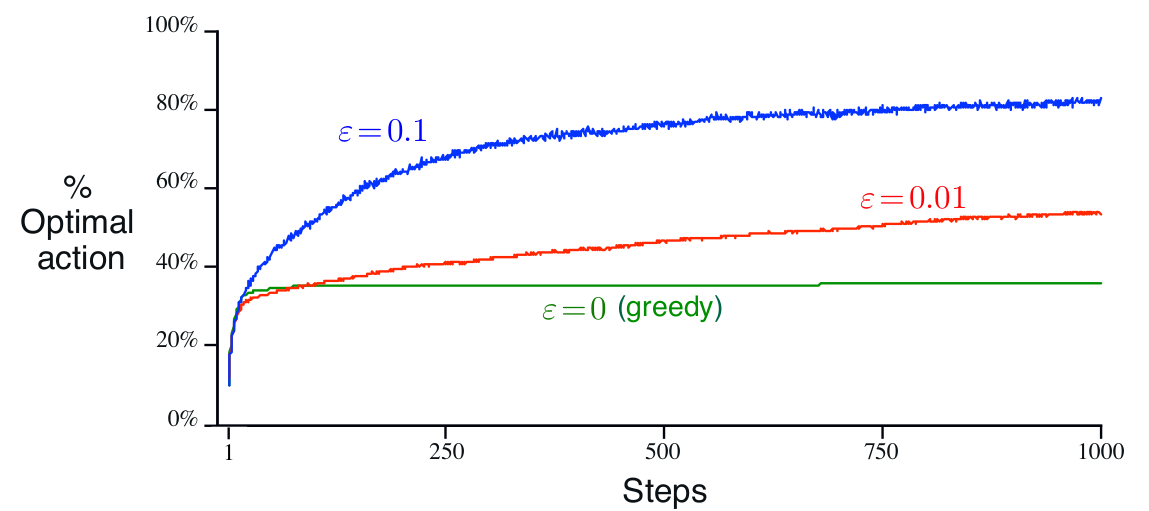
\includegraphics[scale=0.35]{images/eps_vs_optAction.png}
    \caption{Average performance of three agents using different $\epsilon$.  The data is averaged over 2000 runs.  Figure from \textit{Reinforcement Learning: An Introduction} by Sutton and Barto (2018).}
    \label{fig: eps_figure}
\end{figure}

During implementation, $\epsilon$ should decay out as $Q_t(a)$ approaches $q_*(a)$ to ensure knowledge of the agent is being adequately exploited. For non-stationary problems, $\epsilon > 0 \; \forall t$ to ensure other action values have not changed.

Algorithms to solve the \textit{k}-armed bandit problem are easily applied to situations where the concept of state is inert and only the actions are of concern;  a near impossibility in the real world.  

\subsubsection{Contextual Bandit}

A natural extension of the \textit{k}-armed bandit is associative search.  In associative search (sometimes called contextual bandit), different policies are associated with different situations \cite{bartosuttonbrouwer}.  Equation \ref{eq: state-action-value} is the extension of Equation \ref{eq: value} in the associative search problem.

\begin{equation}
    \centering
    q_*(x, u) = \mathbb{E}[R_t | X_t = x, U_t = u]
    \label{eq: state-action-value}
\end{equation}

Associative search is known as the method between \textit{k}-armed bandits and reinforcement learning.  In associative search, the objective is to associate optimal policies to different situations, but only maximizing the \textit{immediate} reward.  Often times, near term sacrifices are required to initiate the trajectory to a large lump sum reward at the terminal state.  For example, heavy capital and time investment is required for University in the short term.  However, the long term gain is so great that it outweighs the short term losses, making going to University an optimal policy for many individuals.

\subsubsection{The Reinforcement Learning Problem}

In order to find the true optimal policy (i.e., policy that returns the greatest rewards over a long time period), the topic of reinforcement learning is developed.  In reinforcement learning, sequential decision making is explored to identify the delayed reward signals from different actions and to ultimately find the optimal policy, $\pi^*$.  

In general terms, reinforcement learning is simply the learning an agent experiences through interactions with the environment.  For added intuition, Figure \ref{fig: simple_rl} shows the generic information flow of reinforcement learning. First, the agent observes some states, $x_t \in \mathcal{X}$, from the environment (some states may be unobservable).  Given $x_t$, the agent performs some actions, $u_t \in \mathcal{U}$ and receives a scalar reward signal, $r_{t+1} \in \mathcal{R}$.  Finally, the environment will transition to a new state, $x_{t+1}$, given probability $P(x_{t+1}, r_{t+1} | x, u)$.

\begin{figure}[h]
    \centering
    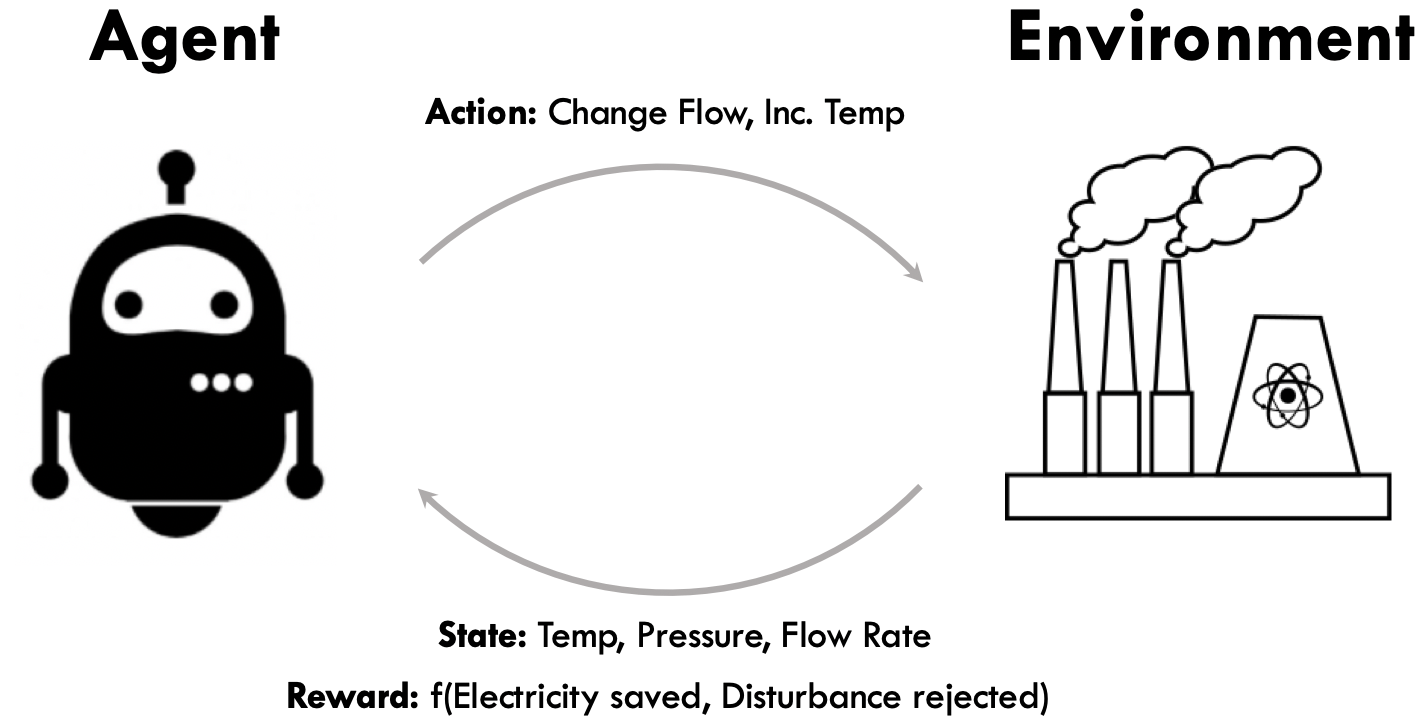
\includegraphics[scale=0.5]{images/RL.png}
    \caption{Basic setup of reinforcement learning where an agent interacts with the environment}
    \label{fig: simple_rl}

\end{figure}

Reinforcement learning consists of the following four elements:

\begin{itemize}
    \item Policy, $\pi$
    \item Reward, $R$
    \item Value Function, $V(s)$
    \item Model (optional), $\dot{x} = Ax + Bu$
\end{itemize}

The policy, $\pi$, of reinforcement learning is a direct mapping from $X \rightarrow U$.  To find the optimal policy, $\pi^*$, the agent is guided by an immediate scalar reward for each interaction (also called \textit{episode}). Policies resulting in higher rewards are more likely to be followed in the future, \textit{mutatis mutandis}.  However, reinforcement learning is concerned with the long term success rather than immediate pleasure. Often times, long term success require short term sacrifice.  Thus, the value function, $V^{\pi}(s)$, is used to describe the long term expected reward under each policy.  Initially, the value function for each state is initialized at zero.  After each episode, the value function will be updated to reflect the new knowledge obtained from the last episode through Equation \ref{eq: value_function}.

\begin{equation}
    \centering
    V(x_t) \leftarrow V(x_t) + \alpha [V(x_{t + 1}) - V(x_t)]
    \label{eq: value_function}
\end{equation}

In Equation \ref{eq: value_function}, $\alpha$ represents the step-size parameter.  That is, how big each update step should be.  Once convergence is achieved for $V(x_t)$, the optimal policy can be described by Equation \ref{eq: opt_policy}.  

\begin{equation}
    \centering
    \pi^*(x) = \argmax_u q_{\pi}(x, u), \; \forall x 
    \label{eq: opt_policy}
\end{equation}

Lastly, reinforcement learning \textit{can} consist of a model. Such cases are called \textit{model-based} reinforcement learning.  The model will be used for planning, and is a way for the agent to plan a control trajectory before they are experienced.  Contrarily, \textit{model-free} reinforcement learning learns \textit{explicitly} through interactions with the environment.

One key topic of reinforcement learning is: \textbf{exploration} vs. \textbf{exploitation}.  At first, the agent must explore to learn the state space, $\mathcal{X}$.  But the agent must know \textit{when} to stop exploring, and start exploiting (i.e., start taking advantage of what is known).  If the agent explores too much, lots of value is lost.  However, if the agent does not explore enough, the current policy may not be optimal and more value is lost long term.  Exploration vs. exploitation is one of the most important topics today in reinforcement learning, and the time to switch from exploration to exploitation will vary between problems.  In control theory, exploration vs. exploitation is known as the conflict between identification (or estimation) and control \cite{explorevexploitcontrol}.  

Another important distinction between different reinforcement learning algorithms is \textbf{on-policy} vs. \textbf{off-policy}.  On-policy methods select actions that maximizes reward given the current knowledge of the agent.  Subsequently, off-policy methods perform exploratory actions for a chance that the explored action offers superior returns to the current best known action.

In the next sub-sections, the three fundamental reinforcement learning methods (Dynamic Programming, Monte Carlo, Temporal-Difference) will be introduced.

\subsection{Dynamic Programming Methods}
\subsubsection{Value-Iteration}
\subsubsection{Policy-Iteration}
\subsection{Monte Carlo Methods}
\subsection{Temporal-Difference Methods}
\subsection{Reinforcement Learning vs. Other "Learnings"}

Machine learning consists of the following four classes: i) Supervised learning, ii) Unsupervised learning, iii) Semi-supervised learning, iv) Reinforcement learning.  Supervised learning is fitting a model to map input data to output data.  The model is initially trained on a set of labeled training data provided by a subject matter expert.  Subsequently, unsupervised learning is used on unlabeled data sets.  The objective of unsupervised learning is to explore the data and identify hidden features. Semi-supervised learning combines the strengths of supervised and unsupervised learning, and is especially useful \cite{machine_learning}.  Often times, industrial data will be partially labelled due to the time and cost associated with data labelling.  For supervised and unsupervised learning, only the labeled and unlabeled data can be used, respectively.  However, all data can be used in semi-supervised learning which allows for maximized data efficiency and increased model performance. Finally, reinforcement learning is a goal-directed learning from interactions with the environment \cite{sutton}.

Reinforcement learning is a unique class of machine learning.  An ideal supervised learning model can only be as good as the subject matter expert providing the labels to the data set, which may not be 100\%.  For example, in a complex control task, the control law is usually highly non-linear. Control experts can try to provide control strategies for such systems, but optimality may not be guaranteed for highly non-linear systems. Also, supervised learning is used to generalize responses for occurrences not present in the data \cite{sutton}.  Reinforcement learning works by directly interacting with the environment \textit{without labels}. Through adequate exploration, reinforcement learning will identify peculiar features to optimally control such problems [citation required].  Reinforcement learning is \textit{similar} to unsupervised learning in terms of identifying hidden structures within the environment.  However, reinforcement learning tries to maximize an internal scalar "reward" signal, rather than purely data mining.

Evolutionary methods, a family of optimization algorithms such as genetic algorithm, are most similar to reinforcement learning.  For a control problem, such methods can apply multiple static policies for different operating regimes \cite{sutton}.  Policy search is conducted by first initiating $k$ random input trajectories of length $N$, generating input matrix $\mathbb{U}_{[k, N]} \in \pi$.  Subsequently, the loss, $J_U$, of each $U$ is calculated based on the objective function.  Input trajectories with the lowest loss move onto the next generation and generates new pseudo-random input trajectories.  This process is repeated until optimal policy, $\pi^*$ is found for each operating regime \cite{ga_for_control}.

Evolutionary methods work well when the policy space is sufficiently small, easy to find, or a lot of time is available for optimization.  The biggest advantage of such methods compared to reinforcement learning is that the whole state does not need to be known.  However, such methods does not capture the reinforcement learning fundamentals of mapping $X \rightarrow U$.  Unlike evolutionary methods, reinforcement learning keeps memory of each indvidual interaction making it a more data efficient approach \cite{sutton}.

%%%%%%%%%%%%%%%%%%%%%%%%%%%%% End Section Intro to RL %%%%%%%%%%%%%%%%%%%%%%%%%%%%%%%%%%%%%%%


%%%%%%%%%%%%%%%%%%%%%%%%%%%%% Begin Section Tabular RL %%%%%%%%%%%%%%%%%%%%%%%%%%%%%%%%%%%%%%

\section{Tabular Q-learning}
\subsection{Introduction to Q-learning}
\subsubsection{Adaptation to Non-Stationary Problems}
\subsubsection{Incremental Implementation}
\subsubsection{Action Selection}
\subsubsection{Exploration in Tabular Q-learning}
\subsubsection{Reward Functions}
\subsubsection{Expected Returns for Different MDPs}

\subsection{Overall Setup}

%%%%%%%%%%%%%%%%%%%%%%%%%%%%% End Section Tabular RL %%%%%%%%%%%%%%%%%%%%%%%%%%%%%%%%%%%%%%%

%%%%%%%%%%%%%%%%%%%%%%% Begin Section Function Approximation %%%%%%%%%%%%%%%%%%%%%%%%%%%%%%%

\section{Function Approximation}
\subsection{Introduction to Function Approximations}
- capture the data of large data set and condense it down into something smaller.
\subsection{Neural Network Basics}
\subsubsection{Neural Network Initialization}
\subsubsection{Gradient Descent Updating}
\subsubsection{Mini-batch Gradient Descent}
\subsubsection{Batch Normalization}
\subsubsection{Regularizations}

%%%%%%%%%%%%%%%%%%%%%%%%% End Section Function Approximation %%%%%%%%%%%%%%%%%%%%%%%%%%%%%%%


%%%%%%%%%%%%%%%%%%%%%%%%%%%%%%%%% Begin Section DDPG %%%%%%%%%%%%%%%%%%%%%%%%%%%%%%%%%%%%%%%

\section{Deep Deterministic Policy Gradient}
\subsection{Actor-Critic Intuition}
\subsection{Actor - Deterministic Policy Gradient}
\subsection{Critic - Deep Q-learning}

\newpage

\subsection{Exploration in DDPG}
\subsubsection{White Exploratory Noise}
\subsubsection{Ornstein-Uhlenbeck Exploratory Noise}
\subsection{Stabilization of Training}
\subsubsection{Experience Replay}
\subsubsection{Target Network}
\subsubsection{Adaptive Batch Gradient Descent}
\subsubsection{Reward Clipping}
\subsection{Input and State Constraints}
\subsection{Training Algorithm}

%%%%%%%%%%%%%%%%%%%%%%%%%%%%%%%%%% End Section DDPG %%%%%%%%%%%%%%%%%%%%%%%%%%%%%%%%%%%%%%%%



%%%%%%%%%%%%%%%%%%%%%%%%%%%%%%%%%%%%%%%%%%%%%%%%%%%%%%%%%%%%%%%%%%%%%%%%%%%%%%%%%%%%%
% Model Predictive Control
%%%%%%%%%%%%%%%%%%%%%%%%%%%%%%%%%%%%%%%%%%%%%%%%%%%%%%%%%%%%%%%%%%%%%%%%%%%%%%%%%%%

%%%%%%%%%%%%%%%%%%%%%%%%%%%%%%%%%%%%%%%%%%%%%%%%%%%%%%%%%%%%%%%%%%%%%%%%%%%%%%%%%%%%%
% Model Predictive Control
%
%
%
%
%%%%%%%%%%%%%%%%%%%%%%%%%%%%%%%%%%%%%%%%%%%%%%%%%%%%%%%%%%%%%%%%%%%%%%%%%%%%%%%%%%%

\section{Model Predictive Control}

Compared to all topics in process control, the concepts of model predictive control (MPC) is perhaps the closest resemblance to modern RL.  MPC is a model-based control strategy (known as a planning method in RL literature) that optimizes the input trajectory of a system by using the functional equation (a function where the unknowns are also functions) generated from the system's state information together with a value function. The performance of MPCs heavily rely on the accuracy of system identification as the input trajectory is solved by extremizing an objective function using mathematical programming (MP) as a function of the process model \cite{mpc}. The objective function is typically given as:
\begin{equation}
    J = \sum\limits^{N}_{i = 1} x_i^TQx_i + \sum\limits^N_{i=1}u_i^TRu_i
    \label{eq:mpc_cost}
\end{equation}
where $N$, $Q$, and $R$ are the prediction horizon and tuning matrices, respectively. Superscript $T$ denotes the transpose operation. $Q$ and $R$ are diagonal matrices and are used to emphasize importance on different state and inputs, respectively. Here, $x$ and $u$ are given as:
\begin{equation}
    x_{sp} - x_i
\end{equation}
\begin{equation}
    u_{ss} - u_i
\end{equation}
where subscripts $sp$ and $ss$ denote the set-point and steady state, respectively. Often times in optimal control, $u_{ss}$ is unknown. In such scenarios, $u$ is given as $\Delta u$ instead, representing a cost in changing the inputs at each step.

Implementation-wise, MPC uses a receding horizon approach where the controller predicts and optimizes for a set amount of steps into the future.  However, only the first control action is implemented.  During the next sampling time, the trajectory is re-optimized and the cycle repeats. The length of the input trajectory and the number of steps the controller predicts into the future are known as the control and prediction horizon, respectively. During design, it is paramount to ensure that both the prediction and control horizons are adequate in length to ensure global optimal solutions.  Intuitively, the prediction and control horizon can be related to the everyday task of driving a car.  It would be very dangerous if we only consider events one second into the future because it would be difficult to react to curves and other road side disturbances; therefore, the prediction and control horizons must be sufficiently long to ensure safe and optimal driving practices. Typically, the control horizon is chosen to be shorter than the prediction horizon due to computational cost and the unimportance of unnecessarily long input trajectories \cite{prediction_horizon}.  One flaw with the receding horizon approach is its extremely expensive online computational cost, especially in large non-linear systems.  

Explicit MPC was developed to mitigate this computational burden by leveraging parametric programming to pre-compute solutions to the optimization problem offline \cite{explicit_MPC}.  During online evaluation, the controller simply looks up the optimal input from a dictionary of pre-computed solutions, making online evaluation extremely fast. This idea is exactly equivalent to RL, where the agent is trained offline (i.e., solves the optimal policies offline), allowing extremely fast online evaluations. 

Ultimately, MPCs provide many advantages compared to classical control strategies.  For example, MPC considers long term planning and identifies the optimal input trajectory rather than the best immediate action.  Furthermore, MPCs have predictive capabilities and can anticipate future events, allowing the controller to plan future control actions accordingly.  A third advantage is that the MP methods used in MPC have been widely demonstrated to handle both input and state constraints relatively successfully.  In modern times, MPCs are often implemented in the supervisory control layer.

The process control hierarchy is shown in Figure \ref{fig:rto_mpc_pid}. Starting from the bottom, the \textit{regulatory controllers} are typically used to ensure stability of the process and directly actuate the process instrumentation.  A common regulatory controller is the Proportional-Integral-Derivative controller (PID). The layers above are known as the \textit{supervisory controllers}. MPC is a common supervisory controller and is classically implemented for regulation or set-point tracking problems exclusively.  Economic objectives of the process were managed by the real time optimization (RTO) layer through steady state optimization \cite{rto}. More recently, control practitioners began to unify the ideas of RTO and MPC into a centralized algorithm called economic model predictive control (EMPC).  Here, the economic objective of the RTO is placed into the objective function of the MPC, allowing for the input trajectory to optimize the economic objective instead \cite{empc2, empc1}. 

\begin{figure}[H]
    \centering
    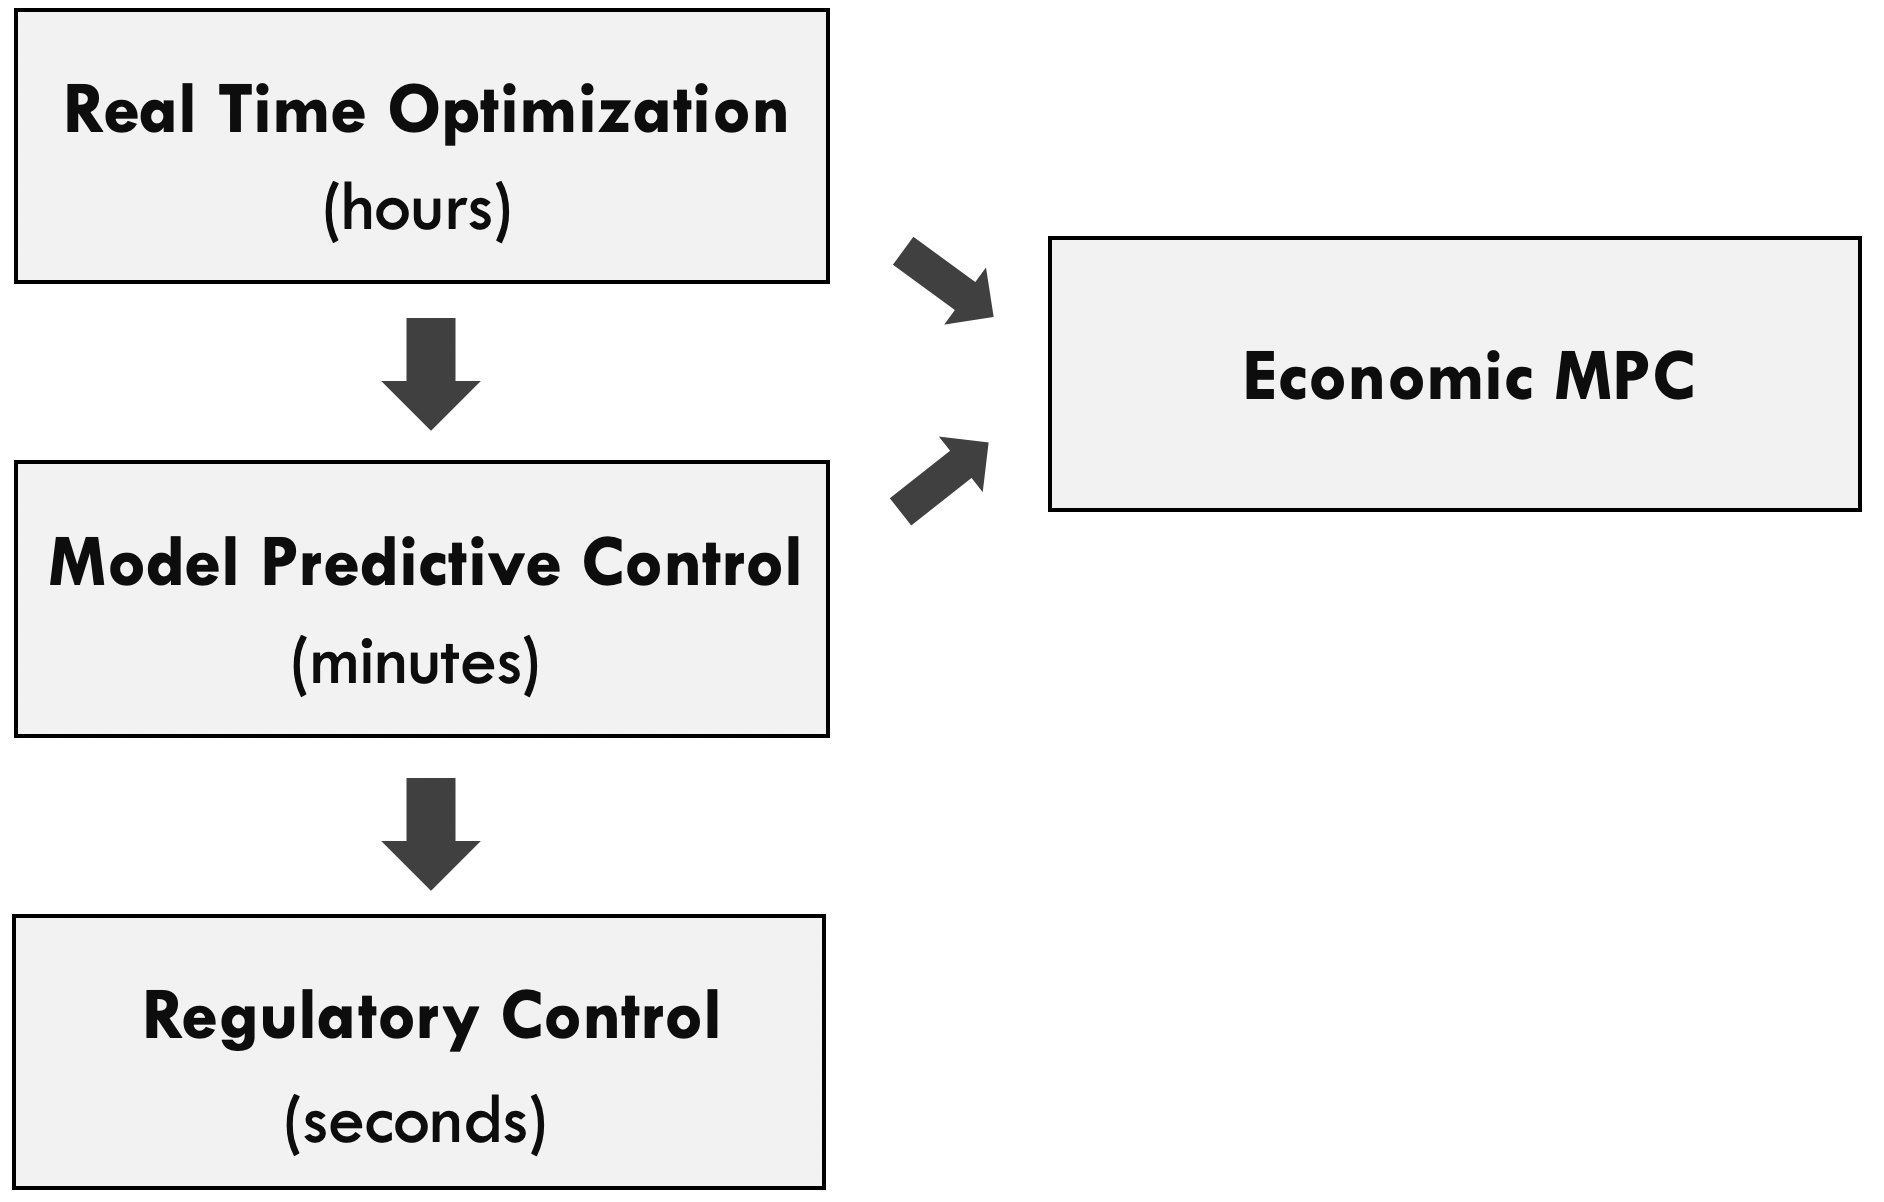
\includegraphics[width=0.5\textwidth]{images/ch1/rto_mpc_pid.jpeg}
    \caption{The traditional control architecture.}
    \label{fig:rto_mpc_pid}
\end{figure}

Comparatively, RL can be described as a general control algorithm and can be used to replace \textit{any} layer in Figure \ref{fig:rto_mpc_pid}. For example, a MPC or PID based RL would have its reward function to be identical as the negative of Equation \ref{eq:mpc_cost}.  In the EMPC case, the reward function of RL would instead be the economic objective.  In Chapter 4, the performance of RL based supervisory controls will be extensively compared to traditional methods on simple and complicated processes. Additionally, the pros and cons of each method will be summarized.
